\documentclass{article}
\usepackage[includeheadfoot,left=1in, right=0.5in, top=0.5in, bottom=0.5in]{geometry}
\usepackage{fancyhdr}
\usepackage{microtype}
\usepackage{lastpage}
%\usepackage{fontspec}
%\setmainfont{Times New Roman}
\usepackage{times}
\usepackage{booktabs}
\usepackage[table]{xcolor}
\usepackage{float}
\usepackage{indentfirst}
\usepackage{url}
\usepackage[pdfborder={0 0 0}]{hyperref}
\usepackage{graphicx}
\usepackage{wrapfig}
\usepackage{caption}
\usepackage{listings}
\usepackage{color}
\usepackage{amsmath}
\usepackage{subcaption}

\date{Fall 2013}
\title{
    \vspace{2in}
    \textmd{\textbf{CS6060- Final}}\\
    \vspace{4in}
}
\author{\textbf{Max Thrun}}

\pagestyle{fancy}
\rhead{Max Thrun}
\lhead{CS6060 - Final}
\rfoot{Page\ \thepage\ of \protect\pageref{LastPage}}
\cfoot{}
\renewcommand\headrulewidth{0.4pt}
\renewcommand\footrulewidth{0.4pt}

\definecolor{sh_comment}{rgb}{0.12, 0.38, 0.18 } %adjusted, in Eclipse: {0.25, 0.42, 0.30 } = #3F6A4D
\definecolor{sh_keyword}{rgb}{0.37, 0.08, 0.25}  % #5F1441
\definecolor{sh_string}{rgb}{0.06, 0.10, 0.98} % #101AF9
\lstset{
    language=C++,
    xleftmargin=.25in,
    xrightmargin=.25in,
    numbers=left,
    numberstyle=\tiny,
    frame=tb,
    showstringspaces=false,
    captionpos=b,
    stringstyle=\color{sh_string},
    keywordstyle = \color{sh_keyword}\bfseries,
    commentstyle=\color{sh_comment}\itshape,
    basicstyle=\tiny\sffamily,
    %numbersep=-5pt,
    belowskip=\baselineskip,
    aboveskip=\baselineskip
}

\makeatletter
\def\lst@PlaceNumber{\llap{\normalfont
                \lst@numberstyle{\the\lst@lineno}\kern\lst@numbersep}}
\makeatother

\newcommand{\mylisting}[3]{
    \lstinputlisting[caption=#3 {\texttt{(\protect\detokenize{#1})}},linerange={#2}]{#1}
}

\parskip = 0.5\baselineskip
\setlength{\belowcaptionskip}{-\baselineskip}

\captionsetup{font=scriptsize}
\captionsetup{labelfont=bf}

\setlength\parindent{0pt}

\begin{document}
\maketitle
\newpage

\section*{Overview}

    The goal of this project was to render a 3D model of my head. A screenshot
    of the end result is shown below.

    \begin{figure}[H]
        \centering
        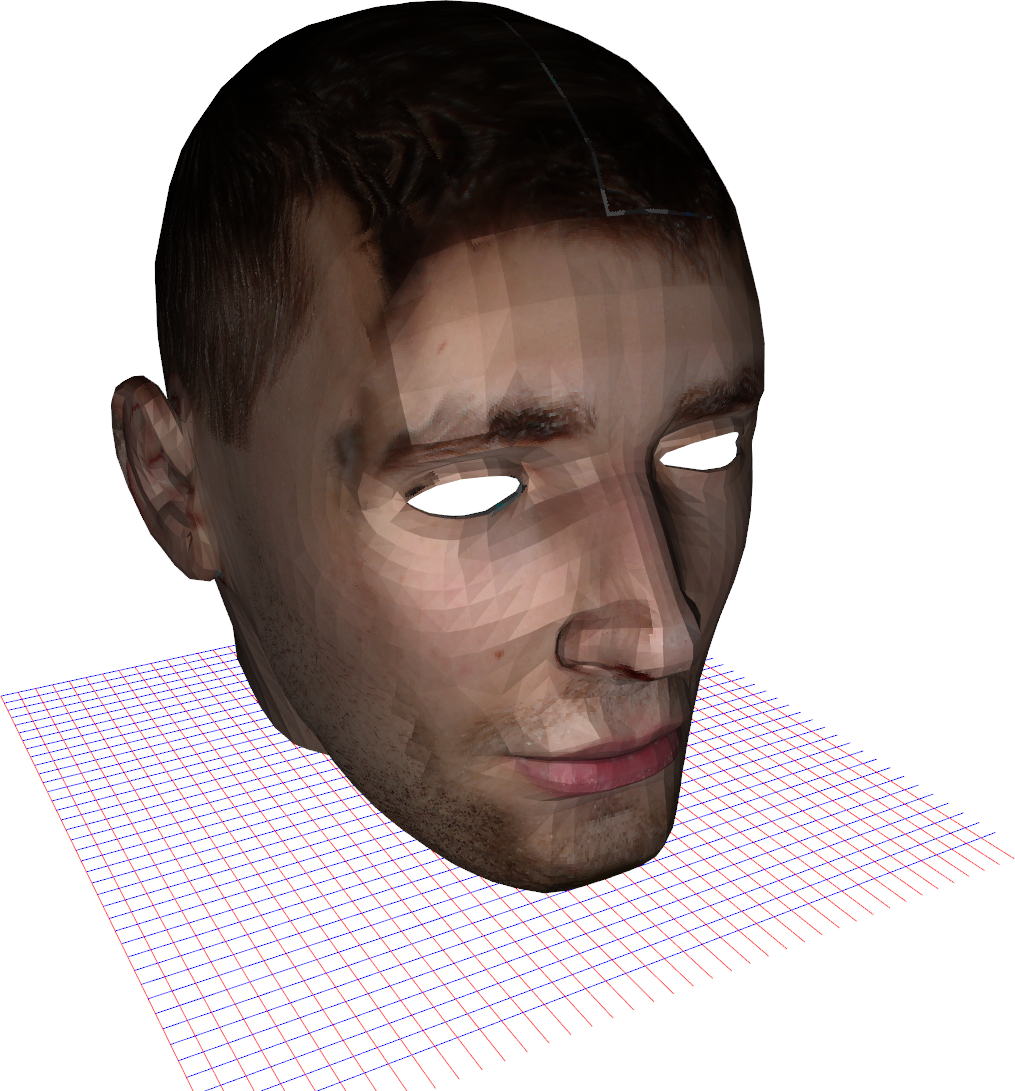
\includegraphics[width=\linewidth]{screenshot}
        \caption{Program Screenshot}
    \end{figure}

    A video demonstation can be found here:
    \url{http://youtu.be/1Sn57Y0Xirw}

    All code and resources can be found here:
    \url{https://github.com/bear24rw/CS6060/tree/master/final}

\newpage
\section*{Head Model}

The first step in this project was to model my head. I didn't have the time or
experience to construct the model from scratch so I found a generic head online
which is shown below.

\vfill
\begin{figure}[H]
    \centering
    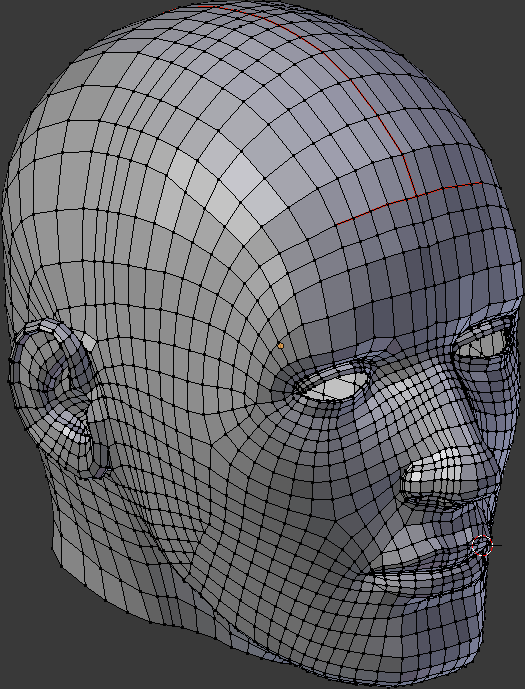
\includegraphics[width=0.8\textwidth]{model.png}
    \caption{Generic 3D Head Model}
\end{figure}
\vfill

\newpage
In order to texture it I first took a front and side image of my head and then
projection mapped them onto the model in Blender.

\begin{figure}[H]
    \centering
    \begin{subfigure}{.5\textwidth}
        \centering
        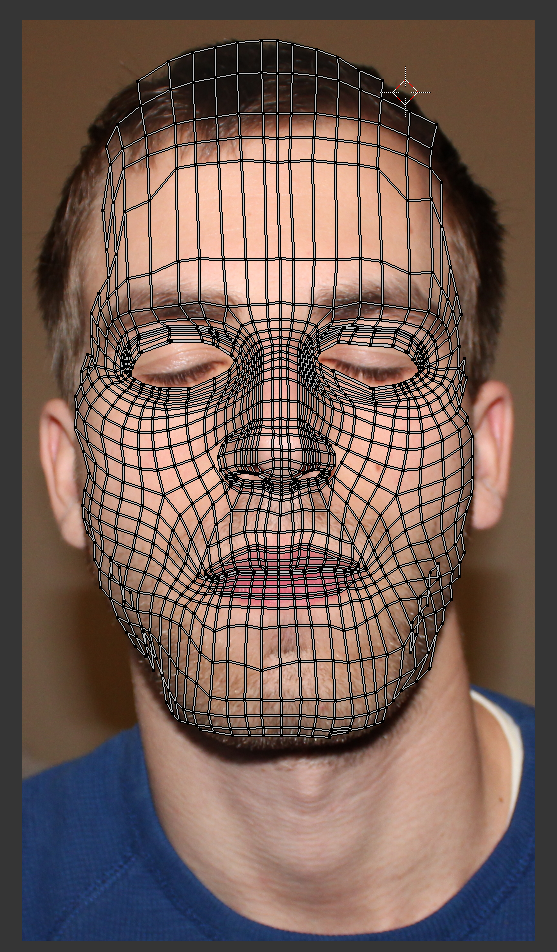
\includegraphics[height=3in]{map_front.png}
        \caption{Front Projection Map}
    \end{subfigure}%
    \begin{subfigure}{.5\textwidth}
        \centering
        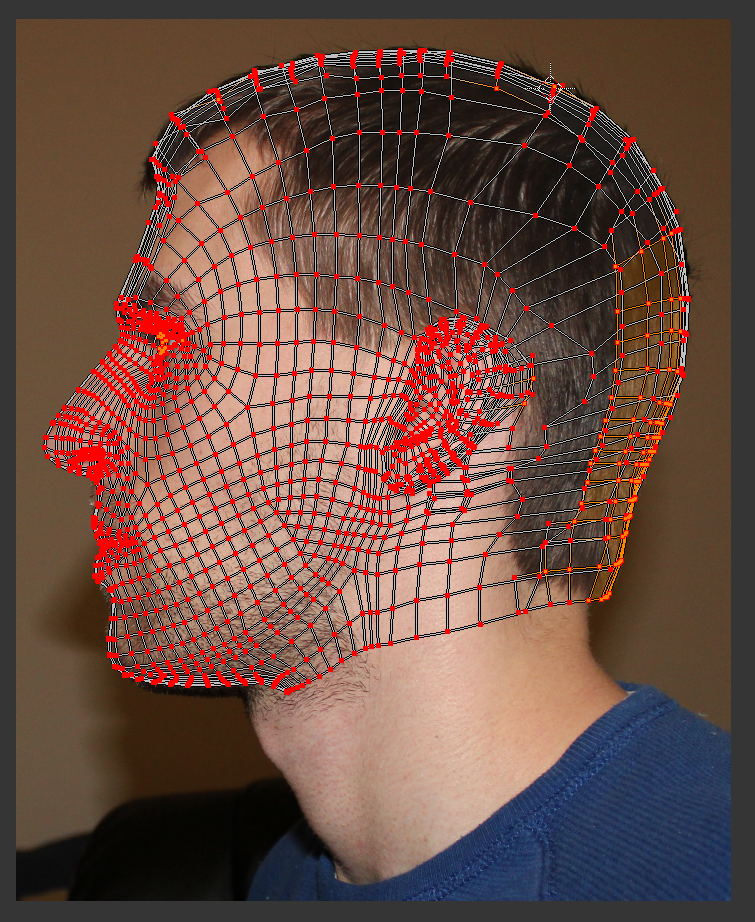
\includegraphics[height=3in]{map_side.png}
        \caption{Side Projection Map}
    \end{subfigure}
    \caption{Projection Texture Mapping}
\end{figure}

The resulting mapping isn't totally perfect since the head
model I used doesn't exactly match my face and I also only
used a front and side image of my face. The images below
show the model pre and post texturing.

\begin{figure}[H]
    \centering
    \begin{minipage}{.5\textwidth}
        \centering
        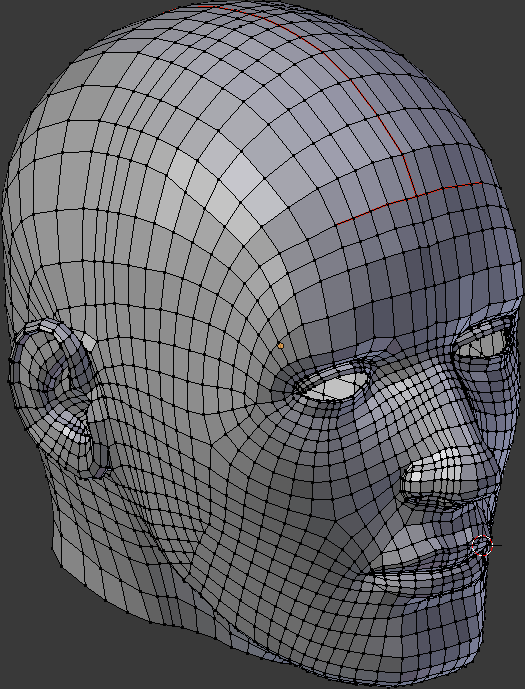
\includegraphics[width=\linewidth]{model.png}
        \captionof{figure}{Untextured Model}
    \end{minipage}%
    \begin{minipage}{.5\textwidth}
        \centering
        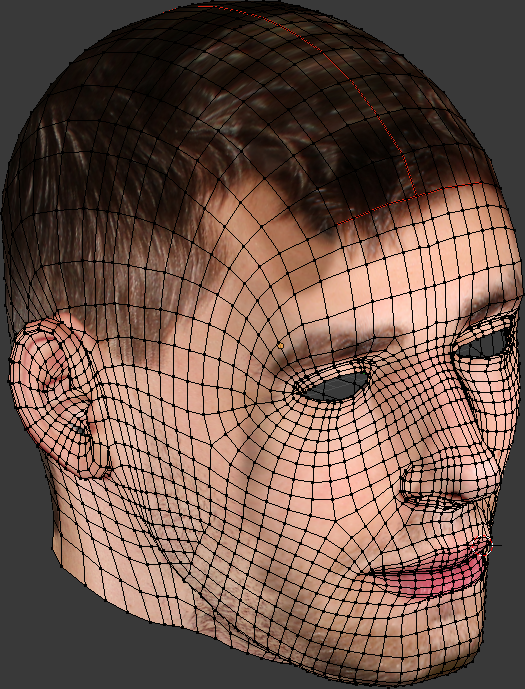
\includegraphics[width=\linewidth]{model_textured.png}
        \captionof{figure}{Textured Model}
    \end{minipage}
\end{figure}

\newpage
I then exported the model as an OBJ file and exported the
texture as a PNG. The final texture is shown below.

\begin{figure}[H]
    \centering
    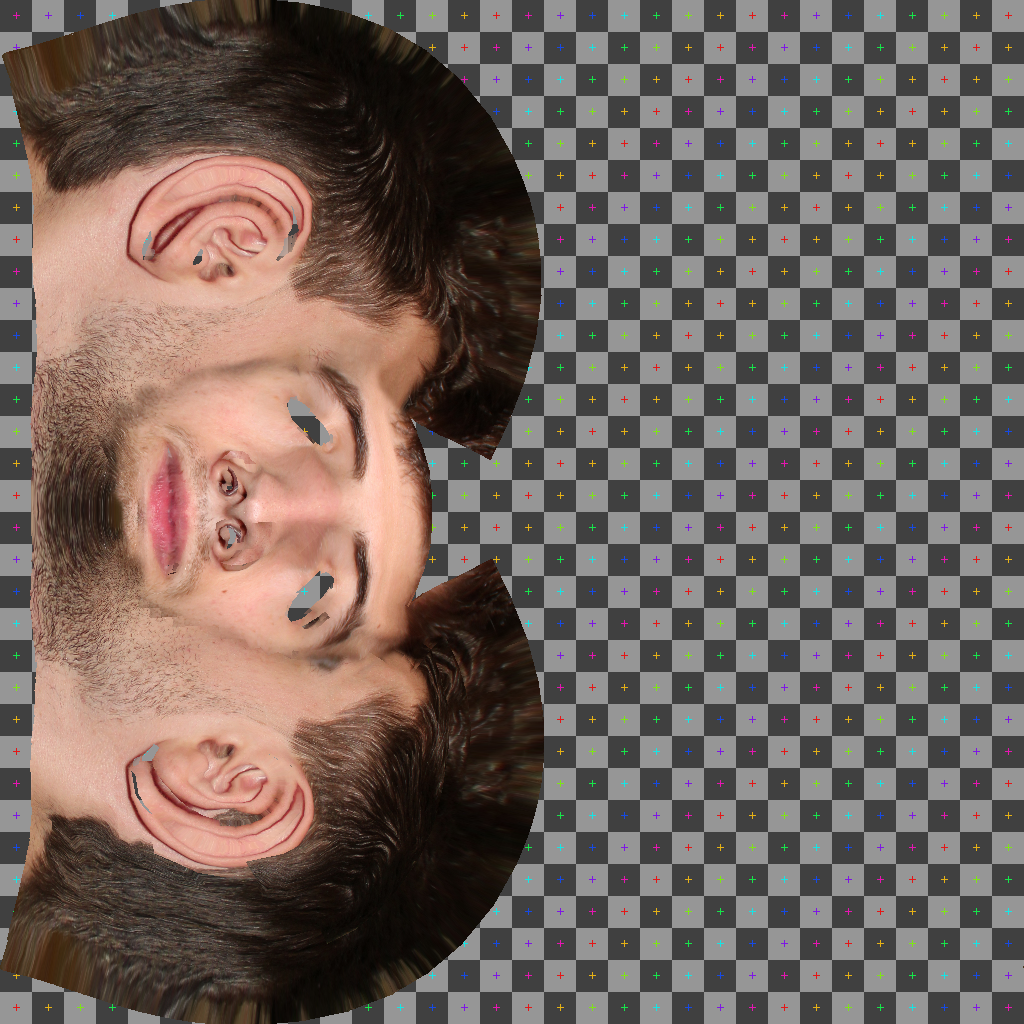
\includegraphics[width=\linewidth]{../assets/uvmap.png}
    \caption{Final Texture}
\end{figure}



\newpage
\section*{Head Rendering}

In order to render the head we first load the shaders and get IDs for
all the uniforms that we will be manipulating.

\mylisting{../code/head.cpp}{21-27}{Load Shader}

For loading the texture we take a shortcut and use the texture functionality
provided by SFML. Since we are just loading a simple 2D texture there is no
need to manually load and bind the texture with raw opengl calls.

\mylisting{../code/head.cpp}{29-29}{Load Texture}


We then create some vectors to hold the vertices, normals, and texture coordinates
for our model and call a helper function to populate them.

\mylisting{../code/head.cpp}{32-35}{Read OBJ}

In order to parse the OBJ file I used the Open Asset Import Library (Assimp).
Assimp takes care of all the dirty work required to parse the OBJ and provides
us with simple lists for the vertices, normals, and uv coordinates. The
following code shows the body of the function which is responsible for opening
the OBJ file with Assimp and populating vectors of GLM objects.

\mylisting{../code/objloader.cpp}{23-65}{OBJ Loading}

\newpage
Next we want to be able to place the bottom of the model at Y=0 and also
center the camera target to the middle of the model. To do this we simply loop through
each vertices of the model and keep track of the lowest one. We will use this offset later
in the render function. The camera is targeted to three fourths of the way up the model which
was determined experimentally to be a nice position.

\mylisting{../code/head.cpp}{32-42}{Calculate model offset}

We then get the shader attribute locations for the vertices, normals, and
texture.  We then create a Vertex Array Object (VAO) which will keep track of
all the bindings and attribute parameters we are about to set. Then, for each
attribute, we generate a vertex buffer, bind it, upload the data for it with
\texttt{glBufferData}, set the parameters for the data with
\texttt{glVertexAttribPointer}, and finally enable the attribute. We also bind
the texture after this.

\mylisting{../code/head.cpp}{46-75}{Setup Bind and Load Buffers}

The rendering function is extremely simple. We first activate the shader
responsible for rendering the head. We then create an identity model matrix
which is first rotated and then translated to achieve the animation and place
the head on the 'ground'. We then send the updated matrices to the shader using
\texttt{glUniformMatrix4fv}. We also update the position of the light to the
position of the camera. Finally we bind our VAO and draw all the elements of
our model.

\mylisting{../code/head.cpp}{80-96}{Render Function}

\section*{Animation}

A simple rotation animation is achieved by keeping track of total rotation
angle. In the main render loop the \texttt{rotation} instance variable is
incremented at a rate of 10 degrees per second. \texttt{delta} is the lapsed
time since the last loop.

\mylisting{../code/main.cpp}{113-114}{Rotation}

The head rendering function, discussed in the previous section, then simply
rotates the model matrix by the number of degrees accumulated in the
\texttt{rotation} variable.

\mylisting{../code/head.cpp}{84-85}{Model Matrix Rotation}

\section*{Lighting}

Lighting is achieved through the combination of diffuse, ambient, and specular components.

The ambient component simply bumps up the brightness of each fragment to
simulate a global indirect light source.

The diffuse component takes into account the distance of the fragment to the
light source and angle of the income light and the fragments normal.

The specular component accounts for the fact that there will be more light
reflecting in the direction that the light intersected the surface.

\mylisting{../code/head_frag.glsl}{18-44}{Head Fragment Shader}

The shader code to achieve these effects was heavily lifted from this tutorial:\\
\url{http://www.opengl-tutorial.org/beginners-tutorials/tutorial-8-basic-shading/}

\section*{Screenshots}

\vfill
\begin{figure}[H]
    \centering
    \begin{minipage}{.5\textwidth}
        \centering
        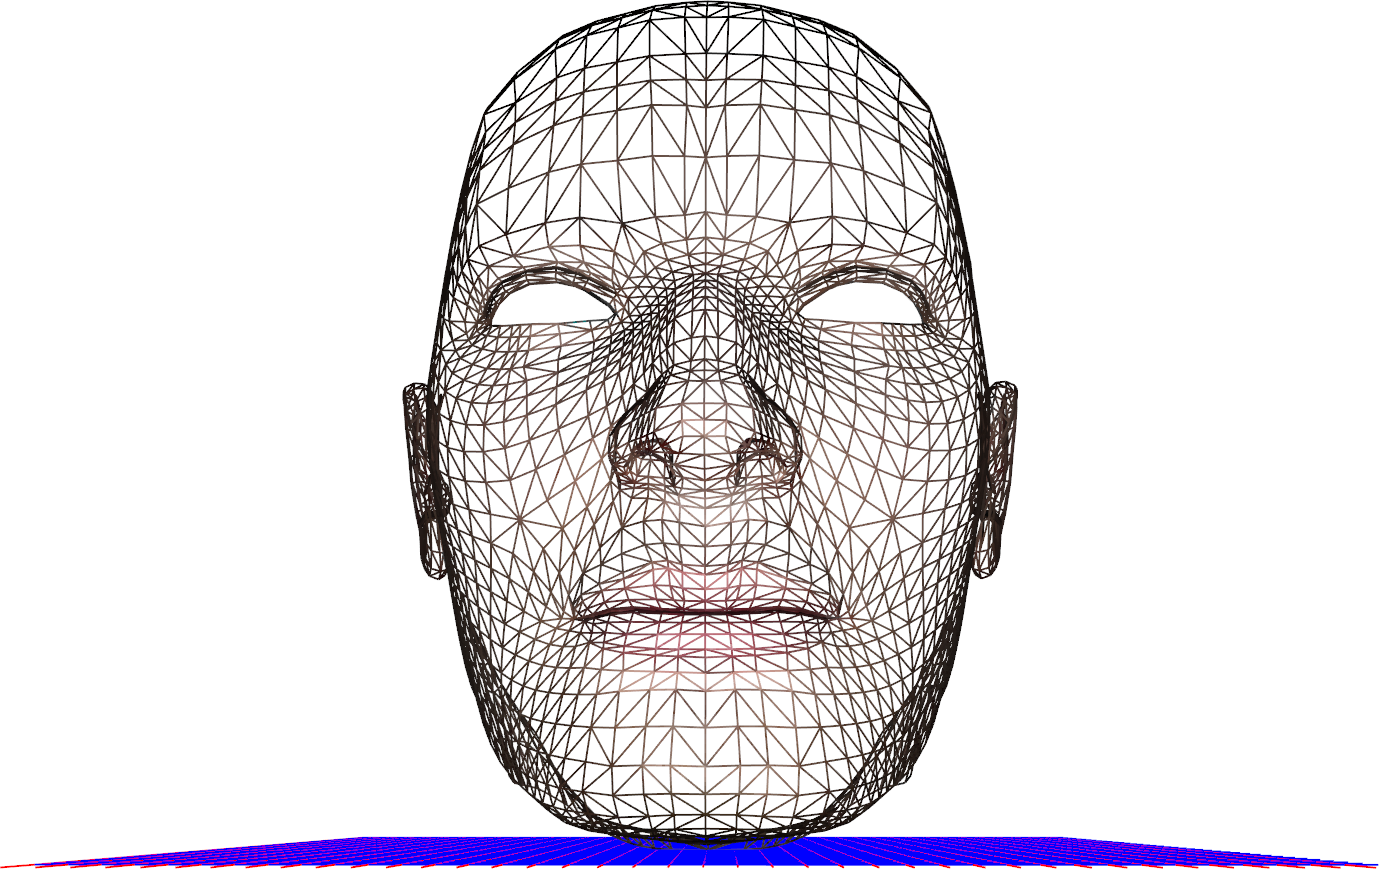
\includegraphics[width=\linewidth]{pic_3.png}
    \end{minipage}%
    \begin{minipage}{.5\textwidth}
        \centering
        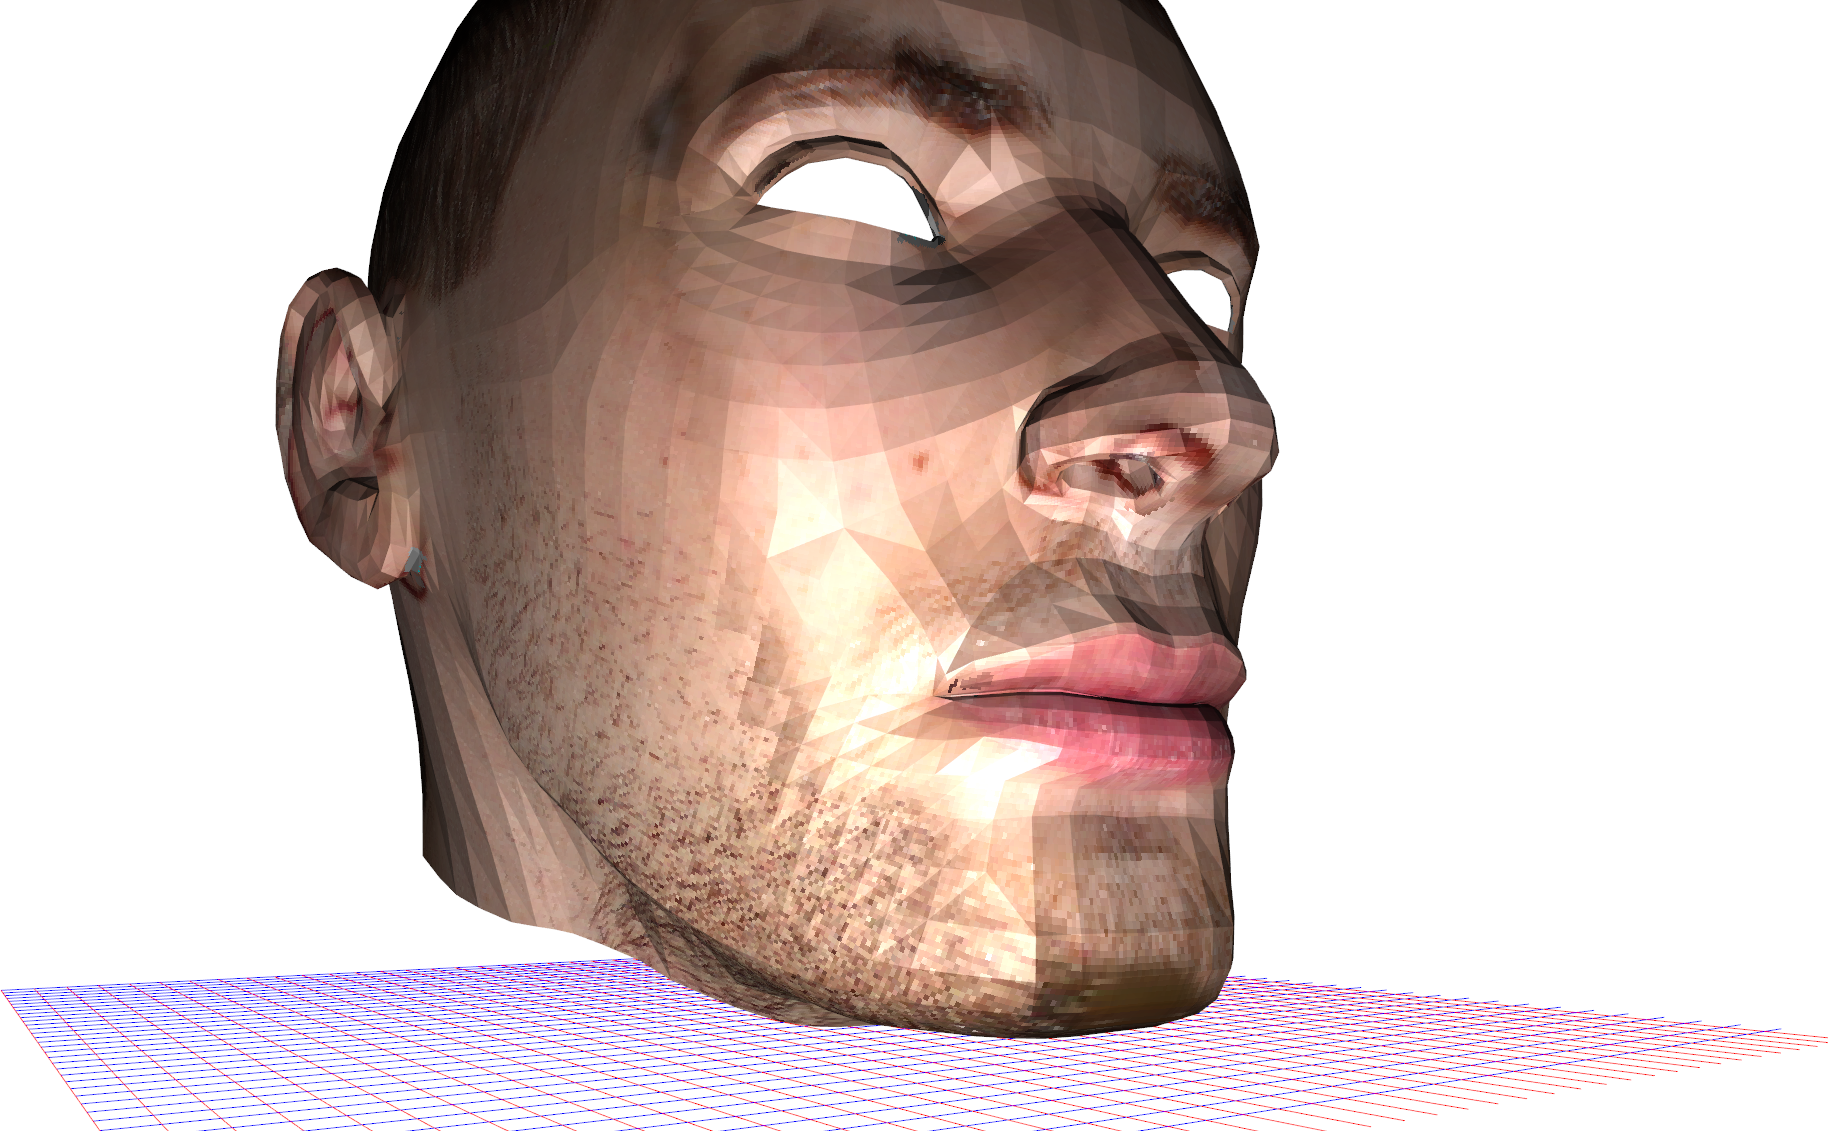
\includegraphics[width=\linewidth]{pic_2.png}
    \end{minipage}

    \vspace{1in}

    \begin{minipage}{.5\textwidth}
        \centering
        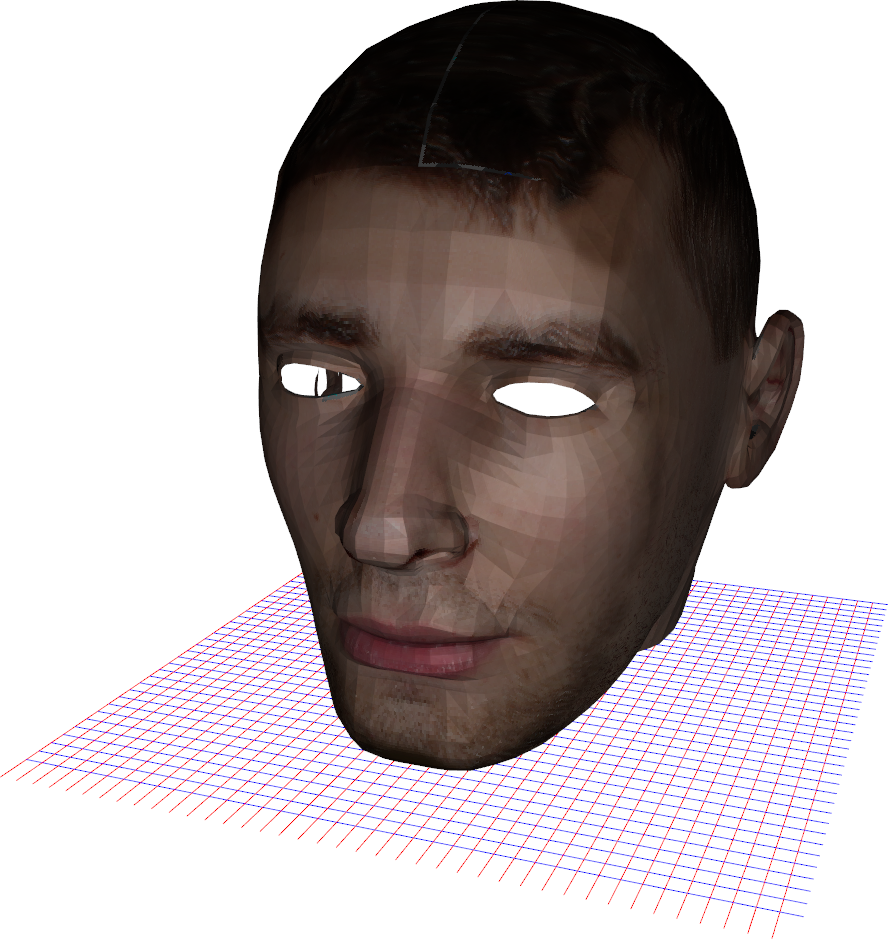
\includegraphics[width=\linewidth]{pic_1.png}
    \end{minipage}%
    \begin{minipage}{.5\textwidth}
        \centering
        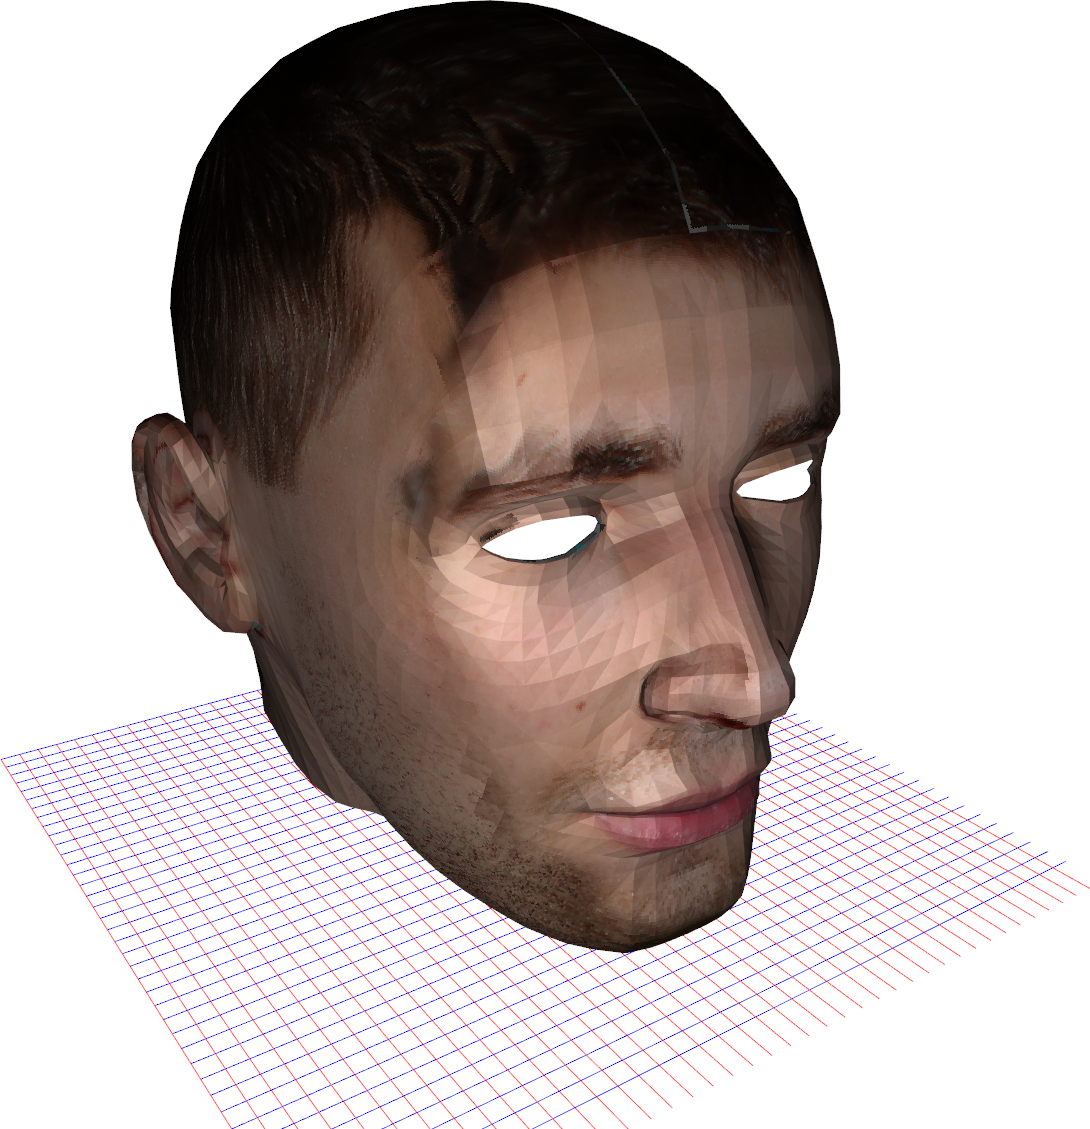
\includegraphics[width=\linewidth]{pic_4.png}
    \end{minipage}
\end{figure}
\vfill

\newpage
\section*{Code}
\mylisting{../code/main.cpp}{}{main}
\mylisting{../code/head.cpp}{}{head}
\mylisting{../code/head.h}{}{head}
\mylisting{../code/grid.cpp}{}{grid}
\mylisting{../code/grid.h}{}{grid}
\mylisting{../code/camera.cpp}{}{camera}
\mylisting{../code/camera.h}{}{camera}
\mylisting{../code/objloader.cpp}{}{objloader}
\mylisting{../code/objloader.h}{}{objloader}
\mylisting{../code/shader.cpp}{}{shader}
\mylisting{../code/shader.h}{}{shader}
\mylisting{../code/head_vert.glsl}{}{head vertex shader}
\mylisting{../code/head_frag.glsl}{}{head fragment shader}
\mylisting{../code/grid_vert.glsl}{}{grid vertex shader}
\mylisting{../code/grid_frag.glsl}{}{grid fragment shader}
\end{document}
